\section{Interpolating $\rho \rightarrow $ R}\label{apx:interp}
OPLIB parameterizes $\kappa_{R}$ as a function of mass density, temperature in keV,
and composition. Type 1 OPAL high temperature opacity tables, which DSEP and
many other stellar evolution programs use, instead parameterizes opacity as a function
of temperature in Kelvin, $R$ (Equation \ref{eqn:Req}), and composition. The
conversion from temperature in keV to Kelvin is trivial (Equation
\ref{eqn:K2Kev}).
\begin{align}\label{eqn:Req}
	R = \frac{\rho}{T_{6}^{3}}
\end{align}
\begin{align}\label{eqn:K2Kev}
	T_{K} = T_{keV} * 11604525.0061657
\end{align}
However, the conversion from mass density to $R$ is more involved. Because $R$
is coupled with both mass density and temperature there there is no way to
directly convert tabulated values of opacity reported in the OPLIB tables to
their equivalents in $R$ space. The TOPS webform does allow for a
density range to be specified at a specific temperature, which allows for R
values to be directly specified. However, issuing a query to the TOPS webform
for not just every composition in a Type 1 OPAL high temperature opacity table
but also every temperature for every composition will increase the number of
calls to the webform by a factor of 70. Therefore, instead of directly
specifying R through the density range we choose to query tables over a
broad temperature and density range and then rotate these tables,
interpolating $\kappa_{R}(\rho,T_{eff}) \rightarrow \kappa_{R}(R,T_{eff})$. 


To preform this rotation we use the \texttt{interp2d} function within
\texttt{scipy}'s \texttt{interpolate} \citep{2020SciPy-NMeth} module to
construct a cubic bivariate B-spline \citep{Dierckx1981} interpolating function
$s$, with a smoothing factor of 0, representing the surface $\kappa_{R}(\rho,
T_{eff})$. For each $R^{i}$ and $T^{j}_{eff}$ reported in type 1 OPAL tables,
we evaluate Equation \ref{eqn:Req} to find $\rho^{ij} =
\rho(T^{j}_{eff},R^{i})$.  Opacities in $T_{eff}$, $R$ space are then inferred
as $\kappa^{ij}_{R}(R^{i},T^{j}_{eff}) = s(\rho^{ij}, T^{j}_{eff})$. 

As first-order validation of this interpolation scheme we can preform a similar
interpolation in the opposite direction, rotating the tables back to
$\kappa_{R}(\rho, T_{eff})$ and then comparing the initial, ``raw'', opacities
to those which have gone through the interpolations process. Figure
\ref{fig:fracdiff} shows the fractional difference between the raw opacities
and a set which have gone through this double interpolation. The red line
denotes $\log(R)=-0.79$ where models near the Jao Gap mass range will
tend to sit for much of their radius. Along the $\log(R)=-0.79$ line the mean
fractional difference is $\langle \delta \rangle = 0.005$ with an uncertainty of
$\sigma_{\langle\delta\rangle} = 0.013$. One point of note is that, because the
initial rotation into $\log(R)$ space also reduces the domain of the opacity
function, interpolation-edge effects which we avoid initially by extending the
domain past what type 1 OPAL tables include cannot be avoided when
interpolating back into $\rho$ space. 

\begin{figure}
	\centering
	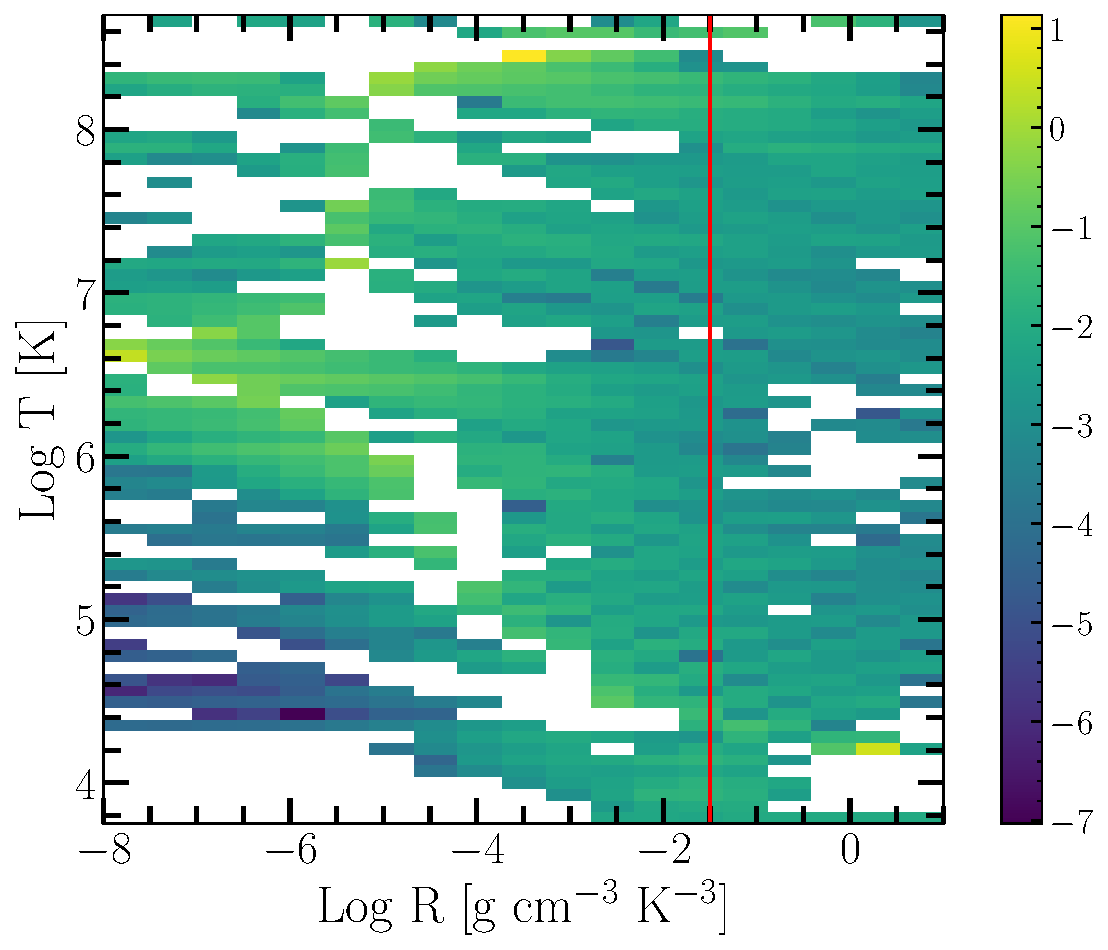
\includegraphics[width=0.45\textwidth]{FractionalDifference.pdf}
	\caption{Log Fractional Difference between opacities in $\kappa_{R}(\rho,
	T_{eff})$ space directly queried from the OPLIB web-form and those which
	have been interpolated into $\log(R)$ space and back. Note that, due to the
	temperature grid of type 1 OPAL tables not aligning perfectly which the temperature
	grid OPLIB uses there may be edge effects where the interpolation is poorly
	constrained. The red line corresponds to $\log(R) = -0.79$ where much of a
	stellar model's radius exists.}
	\label{fig:fracdiff}
\end{figure}

